\documentclass[12pt]{memoir}
\setcounter{tocdepth}{4}
\setcounter{secnumdepth}{3} 
\usepackage[dvipsnames]{xcolor}
\usepackage[utf8]{inputenc}
\usepackage[margin=1in]{geometry}
\usepackage{fancyhdr}
\usepackage{url}
\usepackage{pdfpages}
% \usepackage{biblatex}
\usepackage[
backend=biber,
style=alphabetic,
sorting=ynt
]{biblatex}
\addbibresource{bibliography.bib}

% Images and figure packages
\usepackage{float}
\usepackage{svg}
\usepackage{subcaption}

% Math packages
\usepackage{amssymb}
%\usepackage[cal=boondoxo]{mathalfa}
\usepackage{amsmath}
\usepackage{empheq}
\usepackage{thmtools}
\usepackage{mathtools}
\newtheorem{definition}{Definition}
\newtheorem{theorem}{Theorem}

\declaretheorem[sibling=definition, shaded={rulecolor=black, rulewidth=0.6pt, bgcolor={rgb}{1,1,1}},name=Definition]{boxeddef}
\declaretheorem[sibling=theorem, shaded={rulecolor=black, rulewidth=0.6pt, bgcolor={rgb}{1,1,1}},name=Theorem]{boxedthm}



\usepackage{hyperref}
\hypersetup{
    colorlinks=true,
    linkcolor=blue,
    filecolor=magenta,      
    urlcolor=cyan,
    citecolor=Green,
    pdftitle={Thesis - Danila Mokeev},
    pdfpagemode=FullScreen,
}
\usepackage{underscore}
\usepackage{braket}
\usepackage{afterpage}

% algorithms
\usepackage[linesnumbered,ruled]{algorithm2e}

\setlength\parindent{0pt}

% Commands/shortcuts
% example def of command
% \newcommand{\plusbinomial}[3][2]{(#2 + #3)^#1}
% 3 parameters, with 2 as a default value for #1
\newcommand{\tr}{\text{tr}}
\newcommand{\Tr}{\text{Tr}}
\newcommand{\mb}{\mathbf}
\newcommand{\tb}{\textbf}
\newcommand{\ti}{\textit}
\newcommand{\btheta}{\boldsymbol{\theta}}
\title{Efficient sampling algorithms for Bayesian Quantum Tomography}
\author{Danila Mokeev}
\date{June 2024}

\begin{document}
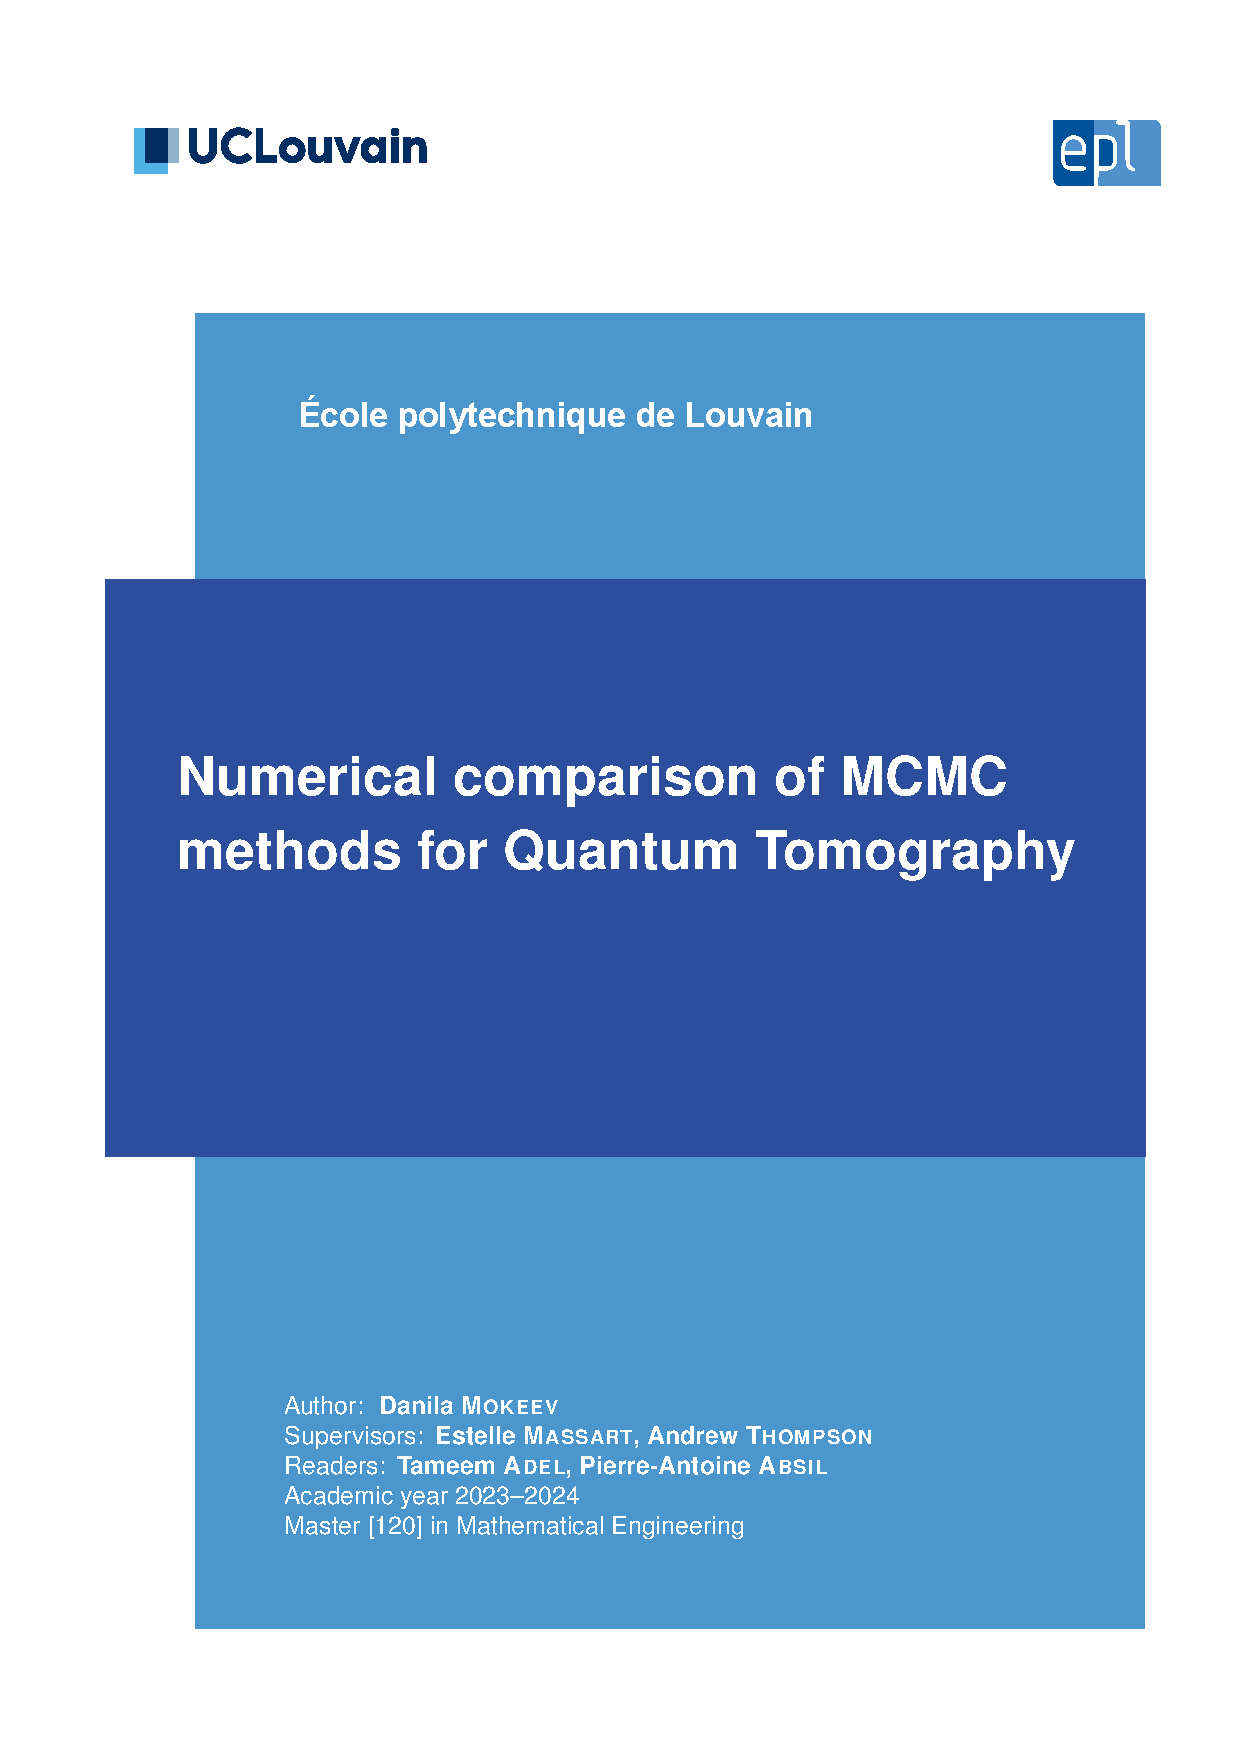
\includepdf[pages={1}]{cover/cover-danila-mokeev.pdf}
\maketitle

\begin{abstract}
    TODO
\end{abstract}

\newpage

\chapter*{Acknowledgements}

\newpage

\tableofcontents*

\newpage

\chapter*{Abbreviations and symbols}
\addcontentsline{toc}{chapter}{\protect\numberline{}Abbreviations and symbols}
\begin{tabular}{ll}
\tb{QT} &  Quantum Tomography \\
\tb{QM} & Quantum Mechanics\\
\tb{prob} & prob-estimator\\
\tb{PL}& Projective Langevin  \\
$\ket{{\psi}}$ & Quantum state $\psi$ in the \ti{bra-ket} formulation\\
$\mb{M^\dagger}$ & Conjugate transponse of matrix $M$\\
$\braket{\mb M}$ & Expected value of a matrix/operator $M$\\
\tb {POVM} & Positive Operator-Valued Measure\\
$\mb{M\otimes N}$ & Kronecker product between matrices $M$ and $N$\\
${U}(a,b)$ & Uniform distribution defined on the open interval $(a,b)$\\
$N(\mu, \sigma^2)$ & Normal distribution with mean $\mu$ and standard derivation $\sigma$
\end{tabular}

\chapter{Introduction}

\section{Motivation and historical context}
%\addcontentsline{toc}{chapter}{\protect\numberline{}Motivation}
\subsection*{Motivation}
A fundamental problem in physics is the reconstruction of the state of a system given measurements describing it. In classical mechanics, this is, at least in theory, always possible due to the deterministic nature of the system. This allows one to make multiple measurements on a system, usually the position and momentum, to exactly determine its state. In Quantum Mechanics (QM), however, the situation is very different: measuring the system settles it, making it impossible to gain more information by repeating measurements. We are also fundamentally limited by what we can measure: the Heisenberg uncertainty principle only allows the measurement of either the position or the momentum, but not both at the same time. Finally, the no-cloning theorem also forbids the system to be copied right before the measurement unless we know the system.\medskip

\textit{Quantum Tomography} (QT) or \textit{Quantum State Tomography} (QST) is a process that allows to reconstruct the state of the system in the context of QM. It tackles the previously described issues by replicating the initial state of the system multiple times, and then measuring once each replica. Note that there is a subtle difference between copying the system and preparing multiple systems with the same steps, as the latter does \textit{not} require any knowledge about the state, only the \textit{steps} necessary to produce it.\medskip

The term ``tomography" means ``to describe an object based on sections, slices" \cite{wiki:tomography}. Many types of tomographies exist and are used in very diverse environments, with notable examples in medical applications, such as Computed Tomography (CT) or Magnetic Resonance Imaging (MRI). QT works in a similar way: we use a set of slices (observables), each of them probing a particular aspect of that state, to reconstruct the quantum state through a tomographic process. An intuitive analogy is the process of shining light on each side of a 3D object, and reconstructing that object from the obtained shadows. This results in an inverse problem, whereby starting from partial and noisy data, we can obtain the true state of the system.

\subsection*{Historical context}
TODO: not sure if this section is needed, if yes then expand\medbreak

QT was first introduced in the 1980s through the term \textit{homodyne tomography} where researchers used light beams to reconstruct the so-called \textit{Wigner} function, a joint quasi-probability density of the position and momentum. This function is derived from the wave function that describes a quantum state, and is probabilistic analog of the phase-space formulation we use in classical mechanics.
\cite{Toninelli19,dariano2003,wignerfunction}.



\section{Quantum Tomography} \label{introduction:quantum-tomography}

%To quote Wikipedia \cite{wiki:QT}: ``Quantum tomography or quantum state tomography is the process by which a quantum state is reconstructed using measurements on an ensemble of identical quantum states". It is therefore an inverse problem, whereby starting from noisy data, we can reconstruct the true state of the system.\\\\
As previously described, the goal of QT is the reconstruction of the system state based on measurements. All of this system information is stored in a matrix, called the \textit{density matrix} $\rho \in \mathbb{C}^{d \times d}$, with $d = 2^n$ and $n$ the number of qubits. Due to the physical properties of the system, this matrix is Hermitian ($\rho = \rho^{\dagger}$), positive semi-definite ($\rho > 0$) and satisfying $\tr(\rho) = 1$. The rank of the matrix also has importance, as it conveys a physical property of the system: pure states are of rank 1, while mixed states are of any rank between 2 and $d$. A pure state is described by the wave function, which is usually represented by a vector, potentially of infinite dimension. Mixed states, on the other hand, are a generalization of pure states and are represented by the density matrix. They correspond to a linear combination of pure states. Pure states correspond to matrices of rank 1, while mixed states are of rank 2 and larger. It is important to note that physicists are mostly interested in density matrices of low rank.\medbreak

QT is based on Born's rule, which links a projective measurement $P_m$ associated to an \textit{observable} $O$ to the probability $p(m)$ of obtaining the associated eigenvalue $m$ given a density matrix $\rho$. This can generally be written as 
\begin{equation}
    p(m) = \tr(\rho P_m)
\end{equation}
By repeating the experiment many times for each observable, we are able to obtain statistically significant estimates for $p(m)$, which combined with the projectors, allows us to estimate the density matrix with any appropriate method.
\section{Overview of existing methods}
We provide first a table summarising existing methods with the papers using them, followed by a more detailed explanation below.  

\begin{center}
    \begin{tabular}{|c|c|}
        \hline
        Method & Papers \\\hline\hline
        Inversion & \cite{meth:linear-inversion:vogel-risken, meth:linear-inversion:RMH, meth:linear-inversion:alquier} \\\hline
        Pauli basis expansion & \cite{Cai-2016}\\\hline
        Maximum Likelihood & \cite{Guta20,meth:ML:BDP,meth:ML:JKMW,meth:ML:Lvovsky,meth:ML:Blume-Kohout,meth:ML:Suzuki,meth:ML:Hradil2004} \\\hline
        Compressed Sensing & \cite{meth:CS:GLFSBE10,meth:CS:Gross-2011, meth:CS:Flammia-2012,meth:CS:Koltchinskii-2011}\\\hline
        Sampling based & \cite{meth:bayesian:smc:Ferrie-2014,meth:bayesian:smc:Kueng-2015, meth:bayesian:sis:Kravtsov-2013}\\\hline
        Metropolis-Hastings based & \cite{MA17,Mai22,LLJL20, meth:bayesian:mh:Blume-Kohout-2010}\\\hline
        Langevin & \cite{meth:bayesian:Langevin:ACMT2024}\\\hline
    \end{tabular}
\end{center}

Well-established methods exist to approximate $\rho$. We can split the existing methods into 5 main categories: inversion, Pauli basis expansion, Maximum Likelihood, Compressed sensing and finally Bayesian methods, which are mostly sampling-based algorithms.\medbreak

Inversion methods are very simple, as they directly rely on the Born rule: $\hat \rho$ is computed by solving the linear system of equations defined by 
\begin{equation*} \label{eq:inversion-method}
        \forall a \in \mathcal{A},\forall s \in \mathcal{S}: \, \hat p_{a,s} = \tr(\hat \rho P^a_s)
\end{equation*}
where $\mathcal{A}$ denotes the set of indices for observables, $\mathcal{S}$ the set of indices for projective measurements, $\hat p_{a,s}$ the empirical probability and $P^a_s$ the projector operator. This approach was introduced in \cite{meth:linear-inversion:vogel-risken}, and then used in \cite{meth:linear-inversion:RMH}, but also in \cite{meth:linear-inversion:alquier}, where they additionally use a rank penalization term. This method is easy to understand, however, it returns a matrix $\hat \rho$ which does not satisfy the properties of a density matrix.\medbreak
%and requires the set of observables to be tomographically complete, which is usually the case but limits us, for example, to run any ablation studies related to the number of observables.
% \begin{equation}
%     \hat p_{a,s} = \tr(\hat \rho \cdot P^{a,s})
% \end{equation}
A second approach, introduced in \cite{Cai-2016}, works by estimating the coefficients in the Pauli basis expansion. Indeed, as the observables of interest we use in QT are the Kronecker product of Pauli matrices (which are usually called $\{\sigma_x, \sigma_y, \sigma_z\} \in \mathbb{C}^{2\times 2}$), we can also approximate $\rho$ using the resulting observable as an element of a base. If we have $\mathcal{B} = \{\sigma_b = \sigma_{b_1} \otimes \dots \otimes \sigma_{b_n}, b \in \{I,x,y,z\}^n\}$, then the density matrix $\rho$ can be approximated as 
\begin{equation}
    \rho = \sum_{b\in\{I,x,y,z\}^n} \rho_b \sigma_b
\end{equation}
In case of \cite{Cai-2016}, the coefficients $\rho_b$ are estimated using an average of the measured eigenvalues with each observable.\medbreak

Another common approach used by many \cite{Guta20,meth:ML:BDP,meth:ML:JKMW,meth:ML:Lvovsky,meth:ML:Blume-Kohout,meth:ML:Suzuki,meth:ML:Hradil2004} is Maximum Likelihood (ML) estimation, which tries to maximize an objective function $\mathcal{L}$ to find the best $\rho$ which matches the data. A possible loss function could be 
\begin{equation}
\mathcal{L}(\rho ; \mb{D}) \propto \prod_{a \in \mathcal{A}} \prod_{s \in \mathcal{S}}\left[\tr\left(\rho P_{{s}}^{{a}}\right)\right]^{n_{{a}, {s}}},
\end{equation}
where $n_{a,s}$ is the number of occurences of $s$ in measurements by $a$. The density matrix is calculated as 
\begin{equation}
    \hat \rho_{\text{ML}} = \text{argmin}_{\rho} \;\mathcal{L}(\rho;\mb{D})
\end{equation}
A downside however often mentioned for this method is the cost, notably for $n\geq10$
\medbreak

There is also a certain number of papers \cite{meth:CS:GLFSBE10,meth:CS:Gross-2011, meth:CS:Flammia-2012,meth:CS:Koltchinskii-2011} which treat the problem of solving \ref{eq:inversion-method} as a pure optimization problem, with the extra contraint that not all observables are available (compressed sensing). They are however less relevant to us, as we consider to be in the tomographically complete case.\medbreak

% Based on the Born rule, we can write the problem as $p_{i} = \tr(\rho \cdot P_i)$ where $p_i$ corresponds to the probability of obtaining $P_i$. The notation $P_i$ refers here to an observable, meaning that it will measure the system at a particular state. This can for example be the spin of each qubit (up or down, in either direction \{x,y,z\}).\\\\ 
% The problem is then framed as follows: based on the empirical frequencies $\hat p_i$ and the observables, which are both known, estimate the density matrix $\rho$ (which we call $\hat \rho$). The empirical probabilities $\hat p_i$ are estimated using $m$ independent copies of the system measured with $P_i$. 
% We will usually refer to $m$ as the number of shots.\\\\

% \[
% \hat p_{\mathbf{a,s}} = \cfrac{1}{m}\sum_{i=1}^m \mathbf{1}_{\{R^\mathbf{a}_i = \mathbf{s}\}}
% \]
% \[
% \hat p_{i} = \cfrac{1}{m}\sum_{i=1}^m \mathbf{1}_{}
% \]
% \[
% \hat p_{\mathbf{a,s}} = \tr(\hat \rho \cdot P^{\mb a}_{\mb s})
% \]
% \[
% \hat p_{i} = \tr(\hat \rho \cdot P_i)
% \]

The methods described so far do not make any assumptions about the structure of $\rho$. They may enforce the properties of a density matrix, but not use the low-rank information, with the only exception being papers which include a rank regularization term in the loss function (such as \cite{meth:linear-inversion:alquier}). To tackle this issue, a good idea is to venture into Bayesian methods, which naturally define a \textit{prior} on $\rho$. They also have the advantage of providing a distribution over it, rather than a point estimate, as most optimization-based do.\medbreak

Bayesian methods rely on \ti{Bayes} theorem, which states that given data $\mb{D}$, which in our case are the empirical probabilities $p_{a,s}$ and projectors $P^a_s$, and parameters $\theta$, in our case the density matrix $\rho$, we can calculate the posterior distribution $\pi(\rho|\mb{D})$:
\begin{equation}
    \pi(\rho|\mb{D}) \propto \pi(\mb{D}|\rho) \pi(\rho)
\end{equation}
where $Pr(\mb{D}|\rho)$ is the likelihood of $\mb{D}$ given $\rho$ and $\pi(\rho)$ the prior distribution over it. There is also a normalizing term, however it normally omitted as it does not modify the result. Obtaining samples from this posterior is what allows the approximation, and the algorithm used for sampling is the key part in the various approaches. The most common estimator then used is the sample mean, also sometimes called the \ti{Bayesian Mean Estimator} (BME) or the Gibbs estimator:
\begin{equation}
    \hat \rho_{\text{BME}} = \int \hat \rho \pi(\hat \rho|\mathcal D) d\hat \rho
\end{equation}
Markov Chain Monte Carlo (MCMC) methods are a big class of sampling methods and are the common tool of choice. In particular, \cite{MA17,Mai22,LLJL20, meth:bayesian:mh:Blume-Kohout-2010} all propose algorithms derived from the very classical Metropolis-Hastings, an algorithm that performs a random walk from an initial point, with an acceptance/rejection step. There are also other strategies, such as Sequential Monte Carlo (SMC) \cite{meth:bayesian:smc:Ferrie-2014,meth:bayesian:smc:Kueng-2015} or Sequential Importance Sampling \cite{meth:bayesian:sis:Kravtsov-2013}. Finally, there is also a new method introduced in \cite{meth:bayesian:Langevin:ACMT2024}, where the authors use the gradient information from the posterior, resulting in Langevin Sampling. This technique provides faster convergence times.\medbreak

The work in the thesis will focus on the prob-estimator introduced in \cite{MA17}, as well as the projected Langevin approach introduced in \cite{meth:bayesian:Langevin:ACMT2024}. They differ in the algorithms they use, Metropolis-Hastings and Langevin sampling, but also in the prior they choose. A complete description of both of these methods is available in section \ref{section:relevant-methods}.

% These methods however have drawbacks, mainly their generic structure, not allowing adding extra information about $\rho$. The inversion method also returns a matrix $\hat \rho$ which does not satisfy the properties of a density matrix, and requires the set of observables to be tomographically complete, which is usually is the case but limits us, for example, to run any ablation studies related to the number of observables.

% This is when the Bayesian framework comes into play: by formulating our problem as 
% $$p(\rho|D) \propto p(D|\rho) p(\rho)$$
% we can add the extra information, for example the fact that $rho$ is low rank. Here, $p(\rho|D)$ is the posterior (distribution of $\rho$ given the data), $p(D|\rho)$ the likelihood and $p(\rho)$ the prior.


% They can either be computed on real hardware by replicating the system $m$ times and measuring with each observable on every copy, or by generating the data. The former requires access to a quantum computer, and for the sake of experiments that will be done, the latter is often enough.


%\section{Markov chain Monte Carlo methods}


\section{Goals and contributions}
In this thesis, our contribution is twofold: first, we investigate how the prob-estimator introduced in \cite{MA17} compares to the projected Langevin algorithm from \cite{meth:bayesian:Langevin:ACMT2024}; second, we try to understand how much impact the used prior has in comparison to the MCMC algorithm that we use to perform the sampling. For the latter, we introduce 2 new algorithms, Metropolis-Hastings with Student-t prior (MHS) and Metropolis-Hastings with Gibbs with Student-t prior (MHGS), which mix the algorithm from \cite{MA17} with the prior from \cite{meth:bayesian:Langevin:ACMT2024}. This allows us to evaluate the advantages that a gradient-based method brings, as well as the effect of a student-t prior on the result. We will focus on providing numerical results, with all the code to reproduce the experiments available in the near future on Github\footnote{\texttt{\url{www.github.com/daqwes/thesis}}}.
\chapter{Background}

\section{Quantum information}
TODO: Not sure about keeping this section \medbreak

Quantum information is a field that explores how information can be encoded and processed using the principles of quantum mechanics. While classical computers perform operations using \textit{bits} (hence either $0$ or $1$), quantum computers operate on $qubits$, which allows for a superposition of bits. This means that a \textit{quantum state} can be in an infinite combination between $0$ and $1$. This property is more clearly explained using probabilities, where the measurement of a qubit in a state will be proportional to the probability associated to it. It is important to note that when we perform the measurement, only one of the states, $0$ or $1$, will be visible.\medskip

This measurement process is very important in quantum mechanics, as contrary to classical mechanics, we can not simply observe the system. There are 4 main properties that limit us: fundamentally, a quantum system is probabilistic - measuring it once does not give any information about the state; in addition, a measurement makes the system collapse - repeating the measurement only yields the same state again; the no-cloning theorem, which does not allow to simply copy the state; finally, the Heisenberg uncertainty principle, which states that either position or momentum can be measured, but not both. Given that, we have to find ways to measure system, and this is where QT fits into the picture.\medbreak

TODO: add another paragraph?
%Another important property that distinguishes quantum mechanics from classical mechanics is the entanglement. This implies that 2 qubits are correlated with each other, and regardless how far they are from each other, the measurement of one 

\section{The qubit}
The $qubit$ is the fundamental unit of computation in quantum information. It contrasts from classical bits by allowing a continuum of states: a linear combination between $0$ and $1$. We usually use the orthonormal basis states with the \textit{bra-ket} formulation to represent it: $\ket 0 = \begin{bmatrix}
    1\\
    0
\end{bmatrix}$ and $\ket 1 = \begin{bmatrix}
    0\\
    1
\end{bmatrix}$. The resulting state $\psi$ is written as follows:
\begin{equation}
    \psi = \alpha \ket 0 + \beta \ket 1 
\end{equation}
where $\alpha,\beta \in \mathbb{C}$ are probability amplitudes, with the constraint that $|\alpha|^2 + |\beta|^2 = 1$. This last equality is needed to satisfy the second axiom of probability, as after the measurement either of outcomes must be observed.\medbreak

A intuitive way to visualise a qubit is to use a \ti{Bloch sphere}. First, we must do a change of coordinates, by going from cartesian to Hopf coordinates. With this in mind, it can be shown that $\ket \psi$ can be rewritten as

\begin{equation}
    \ket \psi = e^{i\gamma}\left( \cos\left(\frac{\theta}{2}\right)\ket 0 + e^{i\phi} \sin\left(\frac{\theta}{2}\ket 1\right)\right)
\end{equation}
with $\theta,\gamma,\phi \in \mathbb{R}$. The term $e^{i\gamma}$ has no observable effects, allowing us to remove it. This leaves us with 2 parameters $\theta$ and $\phi$, which finally allow us to represent the qubit on a sphere:

\begin{figure}[H]
    \centering
    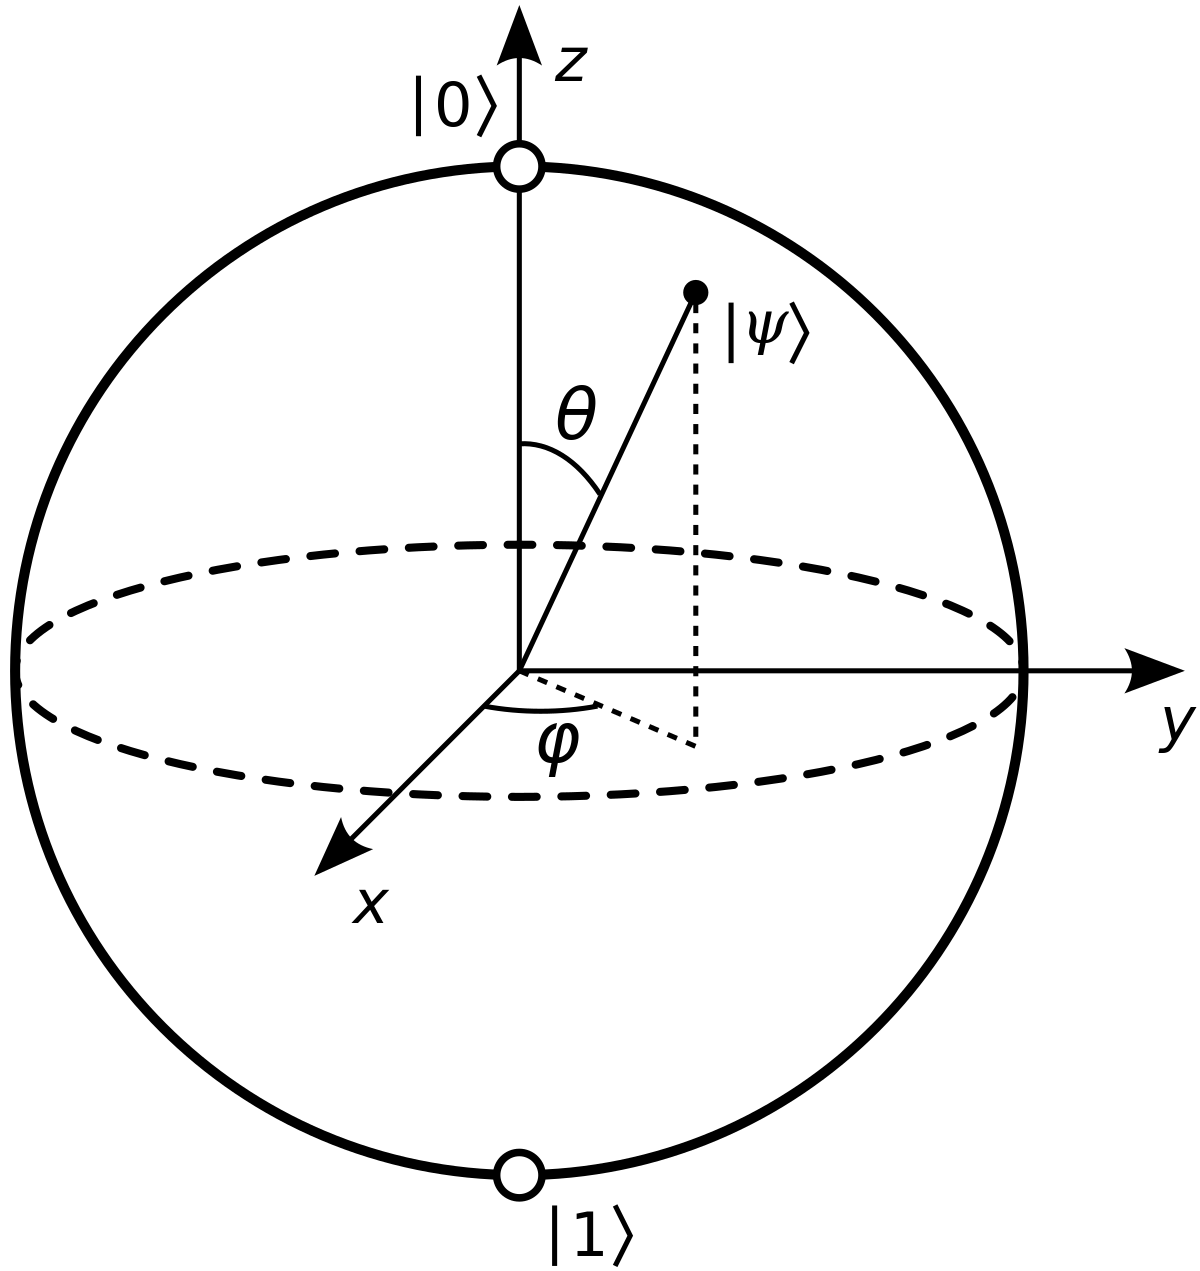
\includegraphics[width=0.3\textwidth]{figures/bloch_sphere.png}
    \caption{Bloch sphere representation of a qubit}
    \label{fig:bloch-sphere}
\end{figure}
While the classical bit only exists in 2 points, the north and south poles, the qubit extends the quantum state to any position on the surface of the cube. \cite{wiki:qubit,book:Nielsen-Chuang-2010}\medbreak

The visual explanation unfortunately fades when we consider multiple qubits: in that case, it is much easier to talk about a $2^n$ dimensional basis. For example, with 2 qubits, 4 basis elements describe a quantum state:

\begin{equation}
    \ket{\phi} = \alpha \ket{00} + \beta \ket{01} + \gamma \ket{10} + \delta \ket{11}
\end{equation}

where $\alpha,\beta,\gamma,\delta \in \mathbb C$ and normalize to 1, and $\phi \in \mathbb{C}^4$.\medbreak

TODO: talk about the EPR state and the entanglement problem?
\section{Quantum Tomography}
As described in \ref{introduction:quantum-tomography}, Quantum Tomography studies the reconstruction of a quantum state described by a density matrix $\rho$. It builds upon the Born rule, which states that given a system state $\ket \psi$ and an observable operator $O$, the probability of occurence of an eigenvalue $m$ of $O$ will be 
\begin{equation}
    p(m) = \braket{\psi | P_m| \psi}
\end{equation}
where $P_m$ is a projection onto the eigenspace of $m$. The system is measured using $O$ with the outcome being an eigenstate $m$.\medbreak

In general, one observable is however not enough as it only measures a specific aspect of a state. We will therefore create a collection of observables $O \in \mathcal{O}$, which will allow us to fully describe our state. In the situation when we have access to the entire set $\mathcal{O}$, we talk about \ti{tomographic completeness}. Of course, doing one measurement with an observable does not provide any information, and in order to obtain any statistically significant estimate for the probability of projector, we measure an ensemble $m$ of identically prepared quantum states for each $O$. \medbreak

In the following sections, we will provide a more thorough mathematical background and describe in more detail the different components that constitute QT.
\subsection{Mathematical description} \label{background:qt:math}

\subsubsection*{Quantum measurement and the Born rule}
The Born rule is a fundamental postulate in QM that connects the wave function to its measurement. It states that ``The probability density of finding a system in a given state, when measured, is proportional to the square of the amplitude of the system's wavefunction at that state" \cite{wiki:born-rule}.\medbreak

A very related postulate is the quantum measurement postulate, which states that quantum measurements are described by a collection $M_m$ of \textit{measurement operators}, which act on the system $\ket \psi$ being measured. The outcome of the measurement corresponds to $m$, and the probability that it occurs is given by
\begin{equation} \label{eq:quantum-measurement}
    p(m) = \braket{\psi|M_m^\dagger M_m|\psi}
\end{equation}
We require the operators to satisfy the \textit{completeness equation}:
\begin{equation}
    \sum_m M_m^\dagger M_m = I
\end{equation}
This equation is equivalent to requiring that the probabilities sum to 1:
\begin{equation}
    1 = \sum_m p(m) = \sum_m \braket{\psi|M_m^\dagger M_m|\psi}
\end{equation}

An example of such a collection is the \textit{computational basis}, represented by $\ket 0$ and $\ket 1$. The resulting matrices are $M_0 = \ket 0 \bra 0$ and $M_1 = \ket 1 \bra 1$, which indeed verify the completeness equation. If we have that $\ket \psi = a \ket 0 + b \ket 1$, then $p(0) = \braket{\psi|M_0^\dagger M_0|\psi} = \braket{\psi|M_0|\psi} = |a|^2$, which a sensible result given the Born rule. The quantum measurement however remains very general, and we usually talk about more specific cases: \textit{POVM} and \textit{projective measurements}.\medskip
    
A \textit{Positive Operator-Valued Measure} (POVM) is a measure whose values $\{F_m\}$ are Hermitian, positive semi-definite operators on a Hilbert space. \cite{wiki:povm} The operators also satisfy the completeness relation, i.e. $\sum_m F_m = I$. This formulation allows to generalize \ref{eq:quantum-measurement}, and rewrite it using the density matrix:

\begin{equation} \label{eq:POVM}
    p(i) = \tr(\rho F_i)
\end{equation}

It can be seen that in case we have a pure state, \ref{eq:POVM} reduces to \ref{eq:quantum-measurement}:
\begin{equation}
    p(i) = \tr(\ket \psi \bra \psi F_i) = \braket{\psi|F_i|\psi}
\end{equation}

An even more specific quantum measurement is the projective measurement. It differs from POVM by forcing the values to be orthogonal projections: if $P_m$ is a projection matrix, then $P_mP_{m'}=\delta_{mm'}P_m$. \medbreak 

The set $\{P_m\}$ relates to an \textit{observable} $O$, which a physical property of a quantum system that can be measured. It can for example be the position, momentum or the spin of a particle. The matrix $O$ is a Hermitian operator, which allows for a simple spectral decomposition:
\begin{equation}
    O = \sum_m m P_m
\end{equation}
where we see that $P_m$ is the projection onto the eigenspace of the eigenvalue $m$  \cite{book:Nielsen-Chuang-2010,wiki:born-rule}. In the context of QT, the most relevant aspect to measure is the spin: in each direction $\{x,y,z\}$, we use a Pauli matrix to probe whether a qubit is spin up $1$ or down (eigenvalue of $1$ or $-1$).
% \begin{equation}
% \begin{split}
%         \braket{M} &= \sum_m m p(m)\\
%          &= \sum_m m \braket{\psi|P_m|\psi}\\
%          &= \braket{\psi|\left(\sum_m m p(m)\right)|\psi}\\
%          &= \braket{\psi|M|\psi}
% \end{split}
% \end{equation}
% where $\braket{M} = E(M)$.\\\\

\subsubsection*{Pure states, mixed states and density matrix}
A pure state is a quantum state that can be represented using a finite or infinite complex vector $\ket \psi$, element of a Hilbert space and of norm 1. Equivalently, it is a state that can not be expressed as a convex combination of other quantum sates \cite{wiki:density-matrix}.\medbreak

A mixed state $\ket \phi$, on the other hand, is a linear combination of pure states $\ket {\psi_j}$. We write 
\begin{equation}
    \ket \phi = \sum_j p_j \ket {\psi_j} 
\end{equation}
where the coefficient $p_j$ is the probability of occurence of $\ket {\psi_j}$. Mixed states usually arise in situations when we do not know from which states our system state is constituted from. This means that we can not anymore represent our system state as a vector, and must resort to a more general form: the density matrix.\medbreak

A \textit{density matrix} $\rho \in \mathbb{C}^{d \times d}$, with $d = 2^n$ and $n$ the number of qubits, is a matrix that represents a general quantum system.
%Such a way to describe a quantum state is only possible when we have a \textit{pure state}, as one ket $\ket \phi$ is enough. In a situation when we do not know from which states our system state is constituted, we must resort to using a matrix formulation. We also know the probabilities $p_j$ associated to these states, describing the mixed state as $\ket \phi = \sum_j p_j \psi_j$.
To calculate this operator, we can use the Born rule seen in \ref{background:qt:math} \cite{wiki:density-matrix}:
\begin{equation}
    p(m) = \sum_j p_j \braket{\psi_j|\Pi_m|\psi_j} = \tr\left[\Pi_m \left(\sum_j p_j \ket{\psi_j}\bra{\psi_j}\right)\right]
\end{equation}
with some projective measurement matrix $\Pi_m$ and associated value $m$. The resulting part on the right corresponds to the density matrix $\rho$:
\begin{equation}
    \rho = \sum_j p_j \ket{\psi_j}\bra{\psi_j}
\end{equation}
Following this derivation, we can see that the properties of a density matrix are that it is Hermitian ($\rho = \rho^{\dagger}$), positive semi-definite ($\rho > 0$) and satisfying $\tr(\rho) = 1$, all of them by construction. The rank of this matrix also allows to easily distinguish between a pure state of rank 1, and a mixed state of any rank between 2 and $2^n$.


\subsection{Data generation}
There are multiple ways through which one can obtain data for quantum tomography: using a real-world dataset is a possibility, however for that, you need access (or need to know someone who has) to a quantum computer. An easier approach is simply to simulate the data. It has its downsides, notably the fact that it may not be representative of true data. In our experiments, however, we will stick to synthetic data as it is very flexible and better suited for algorithm research and numerical experiments due to the low iteration time.\medskip

When using synthetic data generation, 2 main options are usually considered: separate qubit or mixed qubit.


\subsubsection*{Separate qubit data generation}
Separate qubit generation (also called the ``Pauli basis measurements" in \cite{Guta20}) is a process through which we can find the probability associated with an outcome $\mb s = (s_1, s_2 \dots, s_n) \in \mathcal{R}^n := \{-1, 1\}^n $ for an observable $\mb a = (a_1, a_2 \dots, a_n) \in \{x,y,z\}^n$ (we adopt the same notation as in \cite{MA17} here).\medskip

The observable $\sigma_{a_i}$ for a qubit can be in $\{\sigma_x, \sigma_y, \sigma_z\}$, where $\sigma_i \in \mathbb{C}^{2 \times 2}$ is one of the Pauli matrices. These matrices are written as follows:
\begin{equation}
    \sigma_x  = \begin{pmatrix}
        0 & 1\\
        1 & 0
    \end{pmatrix}\quad
    \sigma_y = \begin{pmatrix}
        0 & -i\\
        i & 0
    \end{pmatrix}\quad
    \sigma_z = \begin{pmatrix}
        1 & 0\\
        0 & -1
    \end{pmatrix}
\end{equation}
They distinguish themselves by being Hermitian, unitary and having eigenvalues $\{-1, 1\}$. They correspond to measuring the spin of qubit, an intrinsic property of a particle analogous to angular momentum, along a particular dimension \cite{wiki:pauli-matrices}.
We thus have a total of $3^n$ possible experimental observables and $2^n$ possible outcomes for each observable. Based on the observable and outcome, we can create the operator $P^\mb a_{\mb s} = P^{a_1}_{s_1} \otimes \dots \otimes P^{a_n}_{s_n}$, which corresponds to the projector for this $(\mb a,\mb s)$ pair. The term $P^{a_i}_{s_i}$ corresponds to the orthogonal projection associated to the eigenvalue $s_i$ in the diagonalization of $\sigma_{a_i}$, which in turn can be rewritten as $\sigma_{a_i} = -1P^{a_i}_{-1} + 1P^{a_i}_1$ due to its Hermitian property. Note that under this notation, $\mb a$ and $\mb s$ are both vectors \ti{and} indices. Reminding ourselves of the POVM and Born's rule we saw in \ref{background:qt:math}, we can formulate the main equation as


\begin{equation}
    \forall \mb s \in \mathcal{R}^n, p_{\mb a,\mb s} = \Pr(R^{\mb a} = \mb s) = \tr(\rho P^{\mb a}_{\mb s})
\end{equation}
where $R^\mb{a} \in \mathcal{R}^n$ is the random vector outcome of the experiment $\mb a$ and $p_{\mb a,\mb s}$ the probability linked to that pair. We can see that we recover the projective measurement (or more generally the POVM), only extended to the multi-qubit case by the Kronecker product applied to the projectors $P^{\mb a}_\mb{ s}$.\medbreak

An important element to take into account when working with this method in practice is that, while it the theoretically correct approach, it requires on the order of $6^n = 2^n 3^n$ operations, making it costly.

% Note that there is a slight confusion between the term observable for a qubit (i.e. a Pauli matrix) and an observable to measure the system (in this case the Kronecker product of projection matrices).


\subsubsection*{Mixed qubit data generation}

Mixed qubit data generation (also called ``Pauli observables" in \cite{Guta20}) is an alternative approach, where instead of calculating the probability for each observable/outcome pair, we will directly approximate the expected value linked to this observable. Its calculation is much more straightforward: if we call $A_m$ the observable of which we calculate the expected value, then $A_m = \sigma_{m_1} \otimes \sigma_{m_2} \dots \otimes \sigma_{m_n}$ with $n$ the number of qubits and $m_i$ identifying the Pauli matrix for qubit $i$ for combination $m$ (the notation is the same as in \cite{meth:bayesian:Langevin:ACMT2024}). This results in a total of $4^n$ combinations ($\sigma_{m_i} \in \{I, \sigma_x, \sigma_y, \sigma_z\}$), hence less costly than the separate qubit process.

%\section{Pointwise estimation methods}
\newpage

\section{Markov Chain Monte Carlo methods}
Markov Chain Monte Carlo (MCMC) methods are a class of sampling algorithms. Sampling from a probability distribution is relevant when we want to compute some statistic about it. In most cases, the distribution $\pi(\mb x)$ has high dimensionality as we work in the state of parameters of statistical models. MCMC is particularly important in the context of \ti{Bayesian inference}. In this case, $\pi(\mb x)$ corresponds to the posterior distribution from which we want to sample, and whose probability density function (PDF) is a complex expression. \medbreak

Various methods exist for sampling from simple distributions, the most famous being the inverse transform method, rejection sampling, or importance sampling. All these methods however have drawbacks: inverse transform requires an analytical solution for the cumulative density function (CDF), which is usually not possible to obtain for complex PDFs as it requires a proper integral; rejection sampling and importance sampling do not have this problem, but they suffer from the curse of dimensionality - once your dimension grows, the sampling becomes very inefficient.\medskip

We will now cover several aspects which make up MCMC: Bayesian inference, the theoretical guarantees behind the MCMC methods and finally the 2 main algorithms we will be concerned about in this thesis, Metropolis-Hastings and Langevin sampling.

\subsection{Bayesian inference}\label{section:background:mcmc:bayesian-inference}
As its name suggests, Bayesian inference relies on Bayes theorem. In the context of algorithms, it states that given data $\mb{D}$ and parameters $\boldsymbol{\theta}$, the \textit{posterior} distribution $\pi(\theta|\mb{D})$ is calculated as 
\begin{equation} \label{eq:posterior-with-marginal}
    \pi(\boldsymbol{\theta}|\mb{D}) = \frac{\pi(\mb{D}|\boldsymbol{\theta})\pi(\boldsymbol{\theta})}{\pi(\tb D)} = \frac{\pi(\mb{D}|\boldsymbol{\theta})\pi(\boldsymbol{\theta})}{\int_{\boldsymbol{\theta}} \pi(\mb{D}|\boldsymbol{\theta}) \pi(\boldsymbol{\theta})d\boldsymbol{\theta}}
\end{equation}
where $\pi(\mb{D}|\pi(\boldsymbol{\theta}))$ is the \ti{likelihood} of data given the parameters and $\pi(\theta)$ the \ti{prior} distribution we put on the parameters. The denominator
\begin{equation}
    \pi(\mb{D}) = {\int_{\boldsymbol{\theta}} \pi(\mb{D}|\boldsymbol{\theta}) \pi(\boldsymbol{\theta})d\boldsymbol{\theta}}
\end{equation} 
is called the \ti{marginal}, and corresponds to a normalizing constant. It is in practice intractable to calculate as it involves performing a very high dimensional integral numerically, which is unstable. The good news is that in the context of MCMC methods, the normalizing factor is not important and we can safely remove it. This gives the following posterior:
\begin{equation} \label{eq:posterior-without-marginal}
    \pi(\boldsymbol{\theta}|\mb{D}) \propto {\pi(\mb{D}|\boldsymbol{\theta}) \pi(\boldsymbol{\theta})}
\end{equation}
Getting samples from $\pi(\boldsymbol{\theta}|\mb{D})$ allows us to compute integrals, a technique called Monte Carlo integration. For example, if we have a function $g$ defined on $\mathbb{R}^m$ and we want to approximate its integral on a subset $\Omega \subseteq \mathbb R^m$, we can sample $N$ values uniformly $\{x_i\}_{i=1}^N \in \Omega$ and calculate 
\begin{equation}
    \int_\Omega g(x) dx \approx \frac{1}{N} \sum_{i=1}^{N} g(x_i)
\end{equation}
The law of large numbers ensures that with $N \rightarrow \infty$, the discrete sum converges to the true integral.\cite{wiki:monte-carlo-integration}\medbreak

In statistics, integrals are of particular interest to us as they correspond to expected values. If we have function $f(\boldsymbol{\theta})$ defined on some set $\boldsymbol{\Theta}$, then
\begin{equation}
    \mathbb E_{\boldsymbol \theta \sim \pi(\btheta|\mb{D})}\left(f(\boldsymbol{\theta})\right) = \int_{\boldsymbol{\theta}} f(\boldsymbol{\theta})\pi(\btheta|\mb{D}) d\boldsymbol{\btheta} \approx \frac{1}{N} \sum_{i=1}^{n} f(\boldsymbol{\theta}_i)
\end{equation}
where $\{\boldsymbol{\theta}_i\}^N_{i=1}$ are samples from $\pi(\btheta|\mb{D})$. This allows us to compute estimates for a random variable (with $f(\btheta) = \btheta$), vector or matrix, the last one being the most relevant in QT. In that case, the parameters correspond to the density matrix $\rho$, and the data to the empirical probabilities $\hat p_{a,s}$. By first putting a prior on $\rho$, we can obtain a sample estimate of $\rho$, balanced by the data we have. This is where the term \ti{inference} comes from, as we infer $\rho$ from the data and prior.

\subsection{Theoretical guarantees}\label{section:background:mcmc:theory}
In contrast to Monte Carlo methods where the samples are independent, MCMC builds a \ti{Markov chain} of samples $\btheta^{(1)} \dots \btheta^{(R)}$, which are dependent. As a reminder, a sequence $\mb X^{(1)}, \mb X^{(2)} \dots \mb X^{(R)}$ of random variables is a Markov chain if
\begin{equation}
    \Pr(\mb X^{(r+1)} \in A|\mb x^{(1)}, \dots, \mb x^{(r)}) = \Pr(\mb X^{(r+1)}|\mb x^{(r)})
\end{equation}
where $\mb x^{(i)}$ is a realization of $\mb X^{(i)}$ on domain $A$. One question remains: how can we make sure that samples we obtain from some Markov chain indeed come from the distribution we sample from? In order to answer this, we need to review several properties of Markov chains.\medbreak

A \ti{transition kernel} $k$ is a function that that fully characterizes a Markov chain. It gives the probability of transitioning from one state to another in chain: in the continuous case, this corresponds to conditional function $k(\mb x^{(r+1)}| \mb x^{(r)})$ and the discrete case, it is a transition matrix $P$. We say that our chain in \ti{invariant} to a distribution $\pi(\mb x)$ if 
\begin{equation}
    \pi(\mb x^*) = \int k(\mb x^*|x) \pi(\mb x)d\mb x
\end{equation}
This corresponds to saying that our chain admits a \ti{stationary} distribution, or equivalently that the \ti{marginal} distributions of $\mb X^{(r)}$ and $\mb X^{(r+1)}$ are the same. The distribution $\pi(\mb x)$, called the \ti{target} density, corresponds to the distribution we want to sample from in the context of MCMC. It is important to note that not all chains admit a stationary distribution, and a few properties must be respected. We will cover the discrete case for brevity reasons, but this of course extends to the continuous one \cite{mcmc:slides:Rigon2024Mar,wiki:markov-chain}.
\begin{itemize}
    \item \tb{Irreducibility}: a Markov chain is \ti{irreducible} if it explores the entire sample space, and does not get stuck in local regions. Formally, if $\mb X^{(r)}\in \mathbb{N}$, this corresponds to the condition 
    \begin{equation}
        \Pr(\tau_j < \infty | \mb x^{(0)} = j') > 0\quad \forall j,j' \in \mathbb{N}
    \end{equation} 
    where $\tau_j = \inf\{r\geq 1: \mb X^{(r)} = j\}$ is the first passage time for which the chain is equal to $j$ (defined as $\infty$ if $\mb X^{(r)} \neq j$ for every $r\geq 1$) and $\Pr(\tau_j < \infty | \mb x^{(0)} = j')$ the probability of return to $j$ in a finite number of steps.
    \item \tb{Aperiodicity}: a Markov chain is \ti{aperiodic} if it does not have any deterministic cycles. Formally, we say that a state $j$ is aperiodic if the set $\{r\geq1: [P^r]_{jj} > 0\}$ has no common divisor other than 1 (the matrix $P$ is the ) A chain is aperiodic if all of its states are aperiodic.
    \item \tb{Harris recurrence}:  a Markov chain is \ti{recurrent} if it visits any region of the sample space sufficiently often. Formally, a state $j$ of a discrete irreducible Markov chain is recurrent if and only if
    \begin{equation}
        \Pr(\tau_j < \infty |\mb x^{(0)} = j) = \Pr(\mb X^{(r)} = j \text{ for infinitely many } r | \mb x^{(0)}=j) = 1
    \end{equation}
    In other words, it means that this state is visited infinitely often. If we have all the states that are recurrent, then the chain is called recurrent. If additionally this chain admits an invariant PDF, then it is Harris positive (also called positive recurrent).
    \item \tb{Ergodicity}: a Markov chain in \ti{ergodic} if every state is ergodic. A state $j$ is ergodic if is aperiodic and positive recurrent. Intuitively, this property means that we can reach every state with a probability greater than 0.
\end{itemize}
We can finally state the main result that allows us to use Markov chains for MCMC \cite{mcmc:RobertCasella2004}:
\begin{boxedthm}
    A Markov chain Monte Carlo (MCMC) method converges to a distribution $\pi(\mb x)$ if the underlying Markov chain is ergodic with an equilibrium distribution $f(\mb x) = \pi (\mb x)$.
\end{boxedthm}

A very related theorem that provides a similar guarantee than the law of large number but for Markov chains is the \ti{Ergodic} theorem \cite{mcmc:slides:Rigon2024Mar}:

\begin{boxedthm}
    Let the Markov chain $(\mb X^{(r)})_{r\geq 1}$ be Harris positive with stationary distribution $\pi$, and $g$ be integrable with respect to $\pi$. Then,
    \begin{equation}
        \frac{1}{R}\sum_{r=1}^{R}g(\mb X^{(r)}) \rightarrow \int g(\mb x) \pi(\mb x) d \mb x \quad \text{when } R \rightarrow \infty
    \end{equation} 
    almost surely.
\end{boxedthm}

% \subsection*{MCMC}
% Markov Chain Monte Carlo (MCMC) methods are another class of algorithms to sample from probability distributions.
% %While we can easily sample from standard distributions using methods such as inverse transform sampling, and rejection sampling, we often have no way of sampling from more complex ones, especially those involving a high number of dimensions. 
% MCMC works by constructing a chain of random samples (which are Markovian in nature by being dependent only on the previous one) which at some point are guaranteed to converge to the stationary distribution of the density function of interest. \\\\
% In the usual setting, not all samples are accepted. The probability of acceptance of the next one $x'$ given the current $x$ depends on the ratio $\cfrac{p(x')}{p(x)}$. If the new one is more probable, it is then accepted, otherwise the probability is proportional to the ratio. The class of algorithms that involve this acceptance step are called \textit{adjusted}.\\\\
% In the usual case, MCMC is applied in the context of Bayesian inference. Given the Bayes equation 
% $$
% p(\theta|x) \propto p(x|\theta) p(\theta)
% $$
% we want to obtain samples from the posterior distribution $p(\theta|x)$. This corresponds to getting a distribution for the parameters $\theta$ of our model, given a prior that we have placed over them (our a priori knowledge of how they are distributed) and a likelihood that balances out the prior with data $x$ we have. The Bayes equation in its full form involves a term called the marginal $p(x)$ in the denominator, however as it does depend on the parameters, we do not have to include it.

% %\section{MCMC for Quantum Tomography}
% The samples obtained after MCMC methods are usually used to approximate the distribution of the parameters. In the case of matrix estimation, there are many ways to use these samples. One example is to proceed as in \cite{MA17}, where they construct rank 1 matrices with each sample and then weight them in such a way that only one of the matrices contributes to $\rho$:
% $$
% \hat \rho = \sum_{i=1}^d \gamma_i V_i V_i^{\dagger}
% $$
% The $\gamma_i$ are distributed according to a $\mb{D}ir(\alpha, \dots, \alpha)$ which promotes sparsity among them.


% More formally, given a target distribution $f(x|\theta)$ we can evaluate and proposal distribution  TODO
\subsection{Metropolis-Hastings algorithm}
The \ti{Metropolis-Hastings} (MH) algorithm is the most well-known and used MCMC algorithm. The Markov chain of samples is built by doing a random walk, with an acceptance/rejection step. It works as follows: given that we are currently located at $\mb x$, we will sample a potential candidate $\mb x^*$ from $q(\mb x^*|\mb x)$ where $q$ is called the \ti{proposal} (or \ti{jumping}) distribution. This $q$ is analogous to the kernel we saw in \ref{section:background:mcmc:theory}, although not exactly as we will come back to it later. Next, we will compute the \ti{acceptance} probability of this sample:

\begin{equation}
    \alpha(\mb x^*, \mb x) = \min\left(1, \frac{\pi(\mb x^*) q(\mb x|\mb x^*)}{\pi(\mb x) q(\mb x^*|\mb x)}\right)
\end{equation}
where $\pi(\mb x)$ is the posterior distribution we would like to sample from. Note that we can simplify this criterion in case the proposal density is symmetric ($q(\mb x^*|\mb x) = q(\mb x|\mb x^*)$):
\begin{equation}
    \alpha(\mb x^*, \mb x) = \min\left(1, \frac{\pi(\mb x^*)}{\pi(\mb x)}\right)
\end{equation}
This happens often in practice, as the Gaussian distribution is a common choice of proposal.
A second comment is that, as mentioned in section \ref{section:background:mcmc:bayesian-inference}, the normalizing constant of the posterior does not matter: it gets simplified in the numerator and denominator as it does not depend on $\mb x$, nor $\mb x^*$ (only the data \tb D, see equation \ref{eq:posterior-with-marginal}). \medbreak

After this computation, we will accept $\mb x^*$ with probability $\alpha$. In practice, this involves for example sampling a value $u \sim U(0,1)$, and accepting if $ u \leq \alpha$. This procedure is repeated until the desired number of samples is obtained, with some part of samples that we discard at the beginning. This period is called the \ti{burn-in} period and corresponds to the duration when the samples we obtain are not part of the equilibrium distribution.
We usually talk about convergence when the samples we get seem to come from $\pi$, based on a error-with-respect-to-iterations plot for example. A pseudocode for the algorithm could be:\medbreak

\begin{algorithm}[H]
    \DontPrintSemicolon
    \SetKwInOut{Input}{Input}
    \SetKwInOut{Output}{Output}

    %\underline{Prob-estimator}\;
    \Input{$\mb x_0, T, B$}
    \Output{$\mb x_{B+1}, \mb x_{B+2}, \dots, \mb x_{T}$}
    \For{$t\gets 1:T$}{ 
        Sample $\mb x^* \sim q(\mb x^*|\mb x_{t-1})$\;
        $\alpha = \min\left(1, \frac{\pi(\mb x^*) q(\mb x_{t-1}|\mb x^*)}{\pi(\mb x_{t-1}) q(\mb x^*|\mb x_{t-1})}\right)$\;
        Sample $\mb x^* \sim U(-0.5, 0.5)$\;
        \eIf{$u \leq \alpha$}{
            \tcp*[l]{Accept $\mb x^*$}
            $\mb x_{t} \gets \mb x^*$
        }{
            \tcp*[l]{Reject $\mb x^*$}
            $\mb x_{t} \gets \mb x_{t-1}$
        }
    }
    \caption{Metropolis-Hastings algorithm}
\end{algorithm}\medbreak

We have in section \ref{section:background:mcmc:theory} talked about convergence for Markov chains to the posterior distribution, but have not talked how that would work in practice. A very handy way is to use the \ti{detailed balance} condition.

\begin{boxedthm}
    A Markov chain $(\mb X^{(r)})_{r\geq1}$ with transition kernel $k$ satisfies the detailed balance if there exists a function $f$ such that 
    \begin{equation}
        k(\mb x|\mb x^*) f(\mb x) = k(\mb x^*|\mb x) f(\mb x^*)
    \end{equation}
\end{boxedthm}
In this context, we also talk about \ti{reversibility}:

\begin{boxedthm}
    a Markov chain $(\mb X^{(r)})_{r\geq1}$ is \ti{reversible} if
\begin{equation}
    \Pr(\mb X^{(r)} | \mb X^{(r+1)}) = \Pr(\mb X^{(r+1)} | \mb X^{(r)})
\end{equation}
\end{boxedthm}
Finally, we can reach an important and useful result for MCMC:

\begin{boxedthm}
    if a Markov chain $(\mb X^{(r)})_{r\geq1}$ satisfies the detailed balance with $\pi$ a probability density function, then $\pi$ is the stationary density, and chain is reversible.
\end{boxedthm}

This result means that, as long as we satisfy the detailed balance with our MCMC algorithm, we will converge to the posterior distribution $\pi(\mb)$. In the case of MH, the transition kernel is 
\begin{equation}
    k\left(\boldsymbol{x}^* \mid \boldsymbol{x}\right)=\alpha\left(\boldsymbol{x}^*, \boldsymbol{x}\right) q\left(\boldsymbol{x}^* \mid \boldsymbol{x}\right)+\delta_{\boldsymbol{x}}\left(\boldsymbol{x}^*\right) \int q(\boldsymbol{s} \mid \boldsymbol{x})\{1-\alpha(\boldsymbol{s} \mid \boldsymbol{x})\} \mathrm{d} \boldsymbol{s}
\end{equation}
where $\delta_{\mb x}(\mb x^*)$ is a point mass at $\mb x$. Putting this kernel into the detailed balance condition, one can derive than the equality indeed holds. TODO: derive in appendix? The only element that we have not discussed so far is the ergodicity condition. Altough is depends on $\pi(\mb x)$ and $q$, it is typically true under very mild conditions, which can be checked in, for example, \cite{mcmc:RobertCasella2004}.\medbreak

A final element to take into account with theoretical convergence guarantees is that in practice, the algorithm may take a very long time converge, making it unpractical for real use. In these situations, one could for example investigate different proposals, change the duration of the burn-in period, or even swap MH for another algorithm. Various metrics exist to quantify the convergence, such as the effective sample size or the $\hat R$, but also visual checks, which are very effective. It is also common practice to run several chains from different starting points, and assess the overall performance. More details can be found in \cite{mcmc:gelman2013bayesian}.

\subsection{Gibbs algorithm}
The Gibbs algorithm takes a different approach compared to MH in that it splits the joint distribution $\pi(\mb x) = \pi(x_1, x_2, \dots, x_n)$ with $\mb x \in \mathbb{R}^n$ into one-dimensional conditionals, and then step samples from each conditional $\pi(x_i|\mb x_{-i}) = \pi(x_i|x_1,\dots,  x_{i-1}, x_{i+1}, \dots, x_n)$ iteratively. It can also be generalized to blocks, where instead of sampling from a one-dimensional distribution, we sample from a joint conditional. \medbreak

It is, in its simplest form, an \ti{unadjusted} algorithm, as it does not involve an accept/reject step.
A pseudocode for it can be the following:\medbreak

\begin{algorithm}[H]
    \DontPrintSemicolon
    \SetKwInOut{Input}{Input}
    \SetKwInOut{Output}{Output}

    \Input{$\mb x^{(0)}, T, B$}
    \Output{$\mb x^{(B+1)}, \mb x^{(B+2)}, \dots, \mb x^{(T)}$}
    \For{$t\gets 1:T$}{ 
        $\mb x^{(t)} \gets \mb x^{(t-1)}$\;
        \For{$i\gets 1:n$}{
            \tcp*[l]{Sample from the conditional and set $i$-th element to this value}
            $\mb x_{i}^{(t)} \sim \pi(x_i|\mb x_{-i}^{(t)})$\;
        }
    }
    \caption{Gibbs algorithm}
\end{algorithm}
Note that the inner loop updates the current $x^{(t)}$, and not a copy. This implies that at iteration $i$, we are using the conditioned value set at $i-1$ for $x^{(t)}_{i-1}$, and not the one set at $x^{(t-1)}_{i-1}$.\medbreak

The main advantages of Gibbs sampling is that we do not need to tune the proposal distributions, as well as the fact that all samples are accepted. The downside of course is that we need to be able to derive and sample from the conditional, especially doing so efficiently as otherwise this approach becomes very costly. A more general algorithm, called \textit{Metropolis-within-Gibbs}, involves sampling from the conditional using MH, and in that case this may involve an accept/reject step. In the case of standard Gibbs, we may view the conditionals we sample from as proposal distributions $q(\mb x^*|\mb x)$. This in turn shows us why this algorithm is unadjusted, as the acceptance probability $\alpha$ is always equal to 1 \cite{mcmc:slides:Rigon2024Mar}. If we call $\mb x^* = (x_1^{(t)}, \dots, x_{i}^*, \dots, x^{(t)}_{n})$ and $\mb x = (x_1^{(t)}, \dots, x_{i}^{(t)}, \dots, x^{(t)}_{n})$, then

\begin{equation}
    \alpha(\mb x^*|\mb x) = \frac{\pi(\mb x^*) q(\mb x|\mb x^*)}{\pi(\mb x) q(\mb x^* |\mb x)} = \frac{\pi(x_i^*|\mb x_{-i}^*)\pi(\mb x^*_{-i}) \pi(x_i|\mb x^*_{-i})}{\pi(x_i|\mb x_{-i})\pi(\mb x_{-i}) \pi(x_i^*|\mb x_{-i})} = \frac{\pi( x_i^*|\mb x_{-i})\pi(\mb x_{-i}) \pi(x_i|\mb x_{-i})}{\pi(x_i|\mb x_{-i})\pi(\mb x_{-i}) \pi(x_i^*|\mb x_{-i})} = 1
\end{equation}
where we have used the fact that $\mb x^*_{-i} = \mb x_{-i}$.


\subsection{Unadjusted Langevin algorithm}
One big down-side with Metropolis-Hastings or Gibbs sampling is that they can take a long time to converge, especially in a very high-dimensional setting. The Unadjusted Langevin algorithm (ULA) tackles this problem by using the gradient information about the posterior. The downside, of course, is that we must be able to calculate it, but in the case we can, it can drastically speed-up the convergence. The algorithm draws its name from \ti{Langevin diffusion} (also called \ti{Îto diffusion}), a stochastic differential equation (SDE), which is written as follows:
\begin{equation}
    \mathrm{d}X_t = -\nabla V(x)\mathrm{d}t + \sqrt{2}\mathrm{d}B_t
\end{equation}
where $X_t$ is the position of a particle in a potential $V(x)$ and $B_t$ is the time derivative of the standard Brownian motion. A SDE is a differential equation where one or more of the terms is a stochastic process, and results in a solution which is also a stochastic process. In the case of Langevin diffusion, the solution happens to be a stationary process $p_{\infty}(x) \propto \exp(-V(x))$, which is very handy in the context of MCMC. If we set $V(x) = -\log(\pi(x))$ (we assume a one-dimensional density here), then we can simulate the SDE and obtain samples from $p_\infty = \pi$:
\begin{equation}    
    \mathrm{d}X_t = \nabla \log(\pi(x))\mathrm{d}t + \sqrt{2}\mathrm{d}B_t
\end{equation}

Of course, to simulate, we must discretize the SDE in some way, and in this case \textit{Euler-Maruyama approximation} is what is commonly used. This results in
\begin{equation}
    X^{(k+1)} - X^{(k)} = \tau \nabla \log\pi(X^{(k)}) + \sqrt{2\tau}(B^{k+1} - B^k)
\end{equation}
where $\tau$ is a step size that can be changed over time and $(B^{(k+1)} - B^(k)) \sim N(0, I)$. We can then rewrite it as follows:
\begin{equation}
    X^{(k+1)} = X^(k) + \tau \nabla \log\pi(X^(k)) + \sqrt{2\tau}\xi^(k)
\end{equation}
where $\xi_k \sim N(0, I)$. Note that the true solution can be computed with $X(k\tau)$. The pseudocode can be written as follows (we switch back to using $\mb x \in \mathbb{R}^n$ here):\medbreak
\begin{algorithm}[H]
    \DontPrintSemicolon
    \SetKwInOut{Input}{Input}
    \SetKwInOut{Output}{Output}

    \Input{$\mb x^{(0)}, \tau_{1:T}, T, B$}
    \Output{$\mb x^{(B+1)}, \mb x^{(B+2)}, \dots, \mb x^{(T)}$}
    \For{$t\gets 1:T$}{ 
        $\boldsymbol{\xi}_k \sim N(0, I)$\;
        $\mb x^{(k+1)} = \mb x^{(k)} + \tau_k \nabla \log\pi(\mb x^{(k)}) + \sqrt{2\tau_k}\boldsymbol{\xi}^{(k)}$\;
    }
    \caption{Unadjusted Langevin algorithm}
\end{algorithm}\medbreak

ULA can be seen as noisy gradient ascent, which is why it performs better than MH or Gibbs. By utilizing the gradient information, we are able to sample more often the regions of high density. Note that there also exists a method called \textit{Metropolis-adjusted Langevin algorithm} (MALA), which generalizes this approach with accept/reject step, but we will not go into the details here \cite{mcmc:langenvin-blog:Ansari2024Apr, wiki:MALA}. 

\chapter{Overview of relevant methods} \label{section:relevant-methods}

\section{Prob-estimator}
Introduced in the \cite{MA17} paper, the prob-estimator is a Metropolis-Hastings-based algorithm, where the approximation of $\rho$ is done by a sum of rank 1 matrices and sparse coefficients, leading to a rank 1 approximation:  
\begin{equation}
\hat \rho = \frac{1}{T}\sum_{t=1}^T  \left(
\sum_{i=1}^d \gamma_i^t (V_i^t) (V_i^t)^{\dagger}  
\right)
\end{equation}
This way of approximating $\rho$ is analogous to taking an eigenvector decomposition, except for the fact that we do not require the $V_i$ to be orthonormal (as they are in the case of a decomposition of a symmetric/hermitian matrix). The $\gamma_i$ thus corresponds to an eigenvalue and $V_i$ its associated eigenvector. Because we are promoting sparsity in the coefficients thanks to a Dirichlet prior (this is done by setting all parameters equal to the same small constant), we are also promoting sparsity in the spectrum of $\rho$.\\\\
The MH algorithm is run separately for $\gamma$ and $V$, and can be written as follows:

\begin{algorithm}[H]
    \DontPrintSemicolon
    \SetKwInOut{Input}{Input}
    \SetKwInOut{Output}{Output}

    %\underline{Prob-estimator}\;
    \Input{$\lambda, \alpha, T, V^0$}
    \Output{$\hat \rho $}
    \For{$t\gets 1:T$}{ 
    \tcp*[l]{Update the $\gamma$}
            \For{$i\gets 1:d$}{
            Sample $y \sim U(-0.5, 0.5)$\;
            $\tilde Y_i \gets Y_i^{t-1} \exp (y)$ \;
            $\tilde \gamma_i \gets \tilde Y_i /(\sum_{i=1}^d \tilde Y_i)$\;
            $\tilde Y_i^t \gets \begin{cases}
                \tilde Y_i \hspace{0.96cm} \text{with probability} \min(R(\tilde Y_i, Y_i^{t-1}), 1) \tcp*[l]{$R$ defined below}\\
                Y_i^{t-1} \hspace{0.5cm}\text{otherwise}
            \end{cases}$ \;
            $\forall i, \; \gamma_i^t \gets \tilde Y_i /(\sum(_{j=1}^d \tilde Y_j)$
            }
            
            \tcp*[l]{Update the $V$}
            
            \For{$i\gets 1:d$}{
            
            Sample $V \sim N(\mathbf{0}, \mathbf{I})$\;
      
            $\tilde V_i \gets (V + V_i^{t-1})/||V + V_i^{t-1}||_2$\tcp*[l]{Sample from the unit sphere}\;
            
            $\tilde V_i^t \gets
            \begin{cases}
                \tilde V_i \hspace{0.96cm} \text{with probability} \min(A(\tilde V, V^{t-1}), 1) \tcp*[l]{$A$ defined below}\\
                V_i^{t-1} \hspace{0.5cm}\text{otherwise}
            \end{cases}$
        }
    }
    \caption{Prob-estimator algorithm}
\end{algorithm}

Here, we have that 
$$
\log R(\tilde Y_i, Y_i^{t-1}) = - \lambda \ell^t + \lambda \ell^{t-1} + (\alpha - 1) \log\left(\frac{\tilde Y_i}{Y_t^{t-1}}\right) - \tilde Y_i + Y_i^{t-1}
$$
and 
$$
\log A(\tilde V, V^{t-1}) = -\lambda \ell + \lambda \ell^{t-1} 
$$

The first expression is derived as follows: first, suppose that the proposal distribution is symmetric, in which case it does not take part in the acceptance ratio; then, by Bayes rule, we write
$$
r = \frac{p(\theta'|x)}{p(\theta^{t-1}|x)} = \frac{p(x|\theta') p(\theta')}{p(x|\theta^{t-1})p(\theta^{t-1})}
$$
Here, $\theta$ represents the parameters and $x$ our data. We know the likelihood and prior terms, which are $p(x|\theta) = \exp(-\lambda \ell(\theta, x))$ and $p(\theta) = \cfrac{1}{\Gamma(\alpha)}\theta^{\alpha - 1} \exp(-\theta)$. The paper specifies that instead of working directly on the $\gamma$s, they operate on the $Y$s, which allows them to set a $Gamma(\alpha, 1)$ prior on them. The authors talk about a pseudo-likelihood due to the exponential term, however we will stick to the more general likelihood term for the rest of the document. We then obtain:
$$
r = \frac{\exp(-\lambda \ell') \theta'^{\alpha - 1} \exp(-\theta')}{\exp(-\lambda \ell^{t-1}) \theta_{t-1}^{\alpha - 1} \exp(-\theta^{t-1})}
$$
where we have simplified the $\Gamma$ terms. We can then take the $\log$ of this expression, and replace $\theta = Y_i$:
\begin{align*}
\log(r) &= \log \left( \frac{\exp(-\lambda \ell') \theta'^{\alpha - 1} \exp(-\theta')}{\exp(-\lambda \ell^{t-1}) \theta_{t-1}^{\alpha - 1} \exp(-\theta^{t-1})}\right)\\
&= \log(\exp(-\lambda \ell') \theta'^{\alpha - 1} \exp(-\theta')) - \log(\exp(-\lambda \ell^{t-1}) \theta_{t-1}^{\alpha - 1} \exp(-\theta^{t-1}))\\
&= -\lambda \ell' + \log(\theta'^{\alpha - 1}) - \theta' + \lambda \ell^{t-1} - \log(\theta_{t-1}^{\alpha - 1}) + \theta^{t-1}\\
&= -\lambda \ell' + (\alpha - 1) \log(\tilde Y_i) - \tilde Y_i + \lambda \ell^{t-1} - (\alpha - 1) \log(Y_i) + Y_i^{t-1}\\
&= -\lambda \ell' + \lambda \ell^{t-1} + (\alpha - 1) \log\left(\frac{\tilde Y_i}{Y_i^{t-1}} \right) - \tilde Y_i + Y_i^{t-1}
\end{align*}

One note we can make about this computation is that a fundamental assumption is the symmetricity of the proposal. In our case, however, it does not seem to be the case, as even though we sample from a uniform, we then transform the sample through an exponential. This corresponds in practice to a sample from a pdf of the form $f(x) = 1/x$, which is not symmetric.

\section{Projected Langevin}

Introduced in the \cite{meth:bayesian:Langevin:ACMT2024} paper, the projected Langevin approach is based on an Unadjusted Langevin algorithm. The authors utilize the Burer-Monteiro factorization $\rho = Y Y^*$ with $Y \in \mathbb{C}^{d \times r}$, which corresponds to a low rank (of rank $r$) factorization of $\rho$. This corresponds to considering that the density matrix has a maximum rank of $r$. This also allows us to reduce the dimension of the parameter space from $2d^2$ to $2dr$ by running the MCMC method directly on the $Y$ space. It is important to note that the physical constraints of the problem are still respected, as we assume the $Y$s to belong to the complex hypersphere $C \mathbb{S}^{d\times r} = \{ Y \in \mathbb{C}^{d\times r}: ||Y||_F = 1\}$. The Hermitian and semi-definite positive properties of the density matrix are obtained by construction.\medskip

In addition to the factorization, the paper proposes a new prior, called the spectral scaled Student distribution defined as
\[
\nu_{\theta} (Y) = C_\theta \det(\theta^2I_d + YY^*)^{-(2d+r+2)/2}
\]
This prior is a complex extension of a prior proposed by \cite{Dal20}, where the student-t distribution is a generalization of the Gaussian distribution, allowing for fatter tails. This feature is what promotes sparsity in the eigenvalues of $Y$, favoring a low rank (most samples are close to 0, but occasionally some are large).\\\\
The used likelihood is similar to the prob-estimator, and is written as 
\begin{equation}
L(Y) = \sum^{M}_{i=1} (\hat p_m - \tr(A_mYY^*))^2
\end{equation}
with $A_m$ the Hermitian matrix characterizing the $m^{th}$ experiment and $\hat p_m$ a measured probability.\\\\
Combining these terms, we can obtain a posterior $\hat \nu_{\lambda, \theta}(Y) = \exp(-f_{\lambda, \theta}(Y))$ with
\begin{equation}
    f_{\lambda, \theta}(Y) = \lambda \sum^{M}_{i=1} (\hat p_m - \tr(A_mYY^*))^2 + \cfrac{2d + r + 2}{2}\log \det(\theta^2I_d + YY^*)
\end{equation}
The exponential in this case is useful to us because it allows us to simplify the calculations, as ULA requires us to set the potential $V(x) = -\log(\pi(x))$ where $\pi(x)$ is the posterior from which we want to sample.\\\\ 
The authors also avoid dealing with complex values by using an isomorphism $\psi: \mathbb{C}^{d\times r}\rightarrow \mathbb{R}^{2d\times 2r}$
$$
\psi: M^R + iM^I \rightarrow \frac{1}{\sqrt 2} \begin{pmatrix}
    M^R & - M^I\\
    M^I & M^R
\end{pmatrix}
$$
This results in the following rewrite of $f$:
\[
\tilde f_{\lambda, \theta}(Y) = \lambda \sum^{M}_{i=1} (\hat p_m - \sqrt{2}\tr(\tilde A_m \tilde Y \tilde Y^T))^2 + \cfrac{2d + r + 2}{4}\log \det(\cfrac{\theta^2}{\sqrt 2}I_{2d} + \sqrt 2 \tilde Y \tilde Y^T) + \tilde C
\]
where $\tilde Y = \psi(Y)$ and $\psi(YY^*) = \sqrt{2} \psi(Y)\psi(Y)^T$. We can then also obtain the gradient of $\tilde f_{\lambda, \theta}$
\[
\nabla \tilde f_{\lambda, \theta}(\tilde Y) = -2\sqrt 2 \lambda \sum^{M}_{i=1} (\hat p_m - \sqrt{2}\tr(\tilde A_m \tilde Y \tilde Y^T))^2 (\tilde A_m + \tilde A^T_m)\tilde Y + \cfrac{2d + r + 2}{\theta^2} \left(I_{2d} + \cfrac{2}{\theta^2}\tilde Y \tilde Y^T\right)^{-1} \tilde Y
\]. They also use a trick (Sherman-Morrison-Woodbury formula) to compute the inverse more efficiently:
\[
\left( I_{2d} + \frac{2}{\theta^2} \tilde Y \tilde Y^T \right)^{-1} =  I_{2d} - \tilde Y \left( \frac{\theta^2}{2} I_{2r}+\tilde Y^T \tilde Y \right)^{-1} \tilde Y^T
\]\\\\
Putting all these things together, we can write the resulting algorithm:

\begin{algorithm}[H]
    \DontPrintSemicolon
    \SetKwInOut{Input}{Input}
    \SetKwInOut{Output}{Output}

    %\underline{Prob-estimator}\;
    \Input{$Y_0 \in \mathbb{C}^{d \times r}, \{\eta_k | k\in 1\dots T\}, \beta, \theta, \lambda$}
    \Output{$\tilde Y$}
    $\tilde Y_0 \gets \psi(Y_0)$\;
    \For{$k\gets 1:T$}{ 
        $w_k^R, w_k^I \sim N(0, 1)^{d\times r}$\;
        $w_k \gets w_k^R + i w_k^I$\;
        $\tilde w_k \gets \psi(w_k)$\;
        $\tilde Y_k \gets \tilde Y_{k-1} - \eta_k \nabla f  (\tilde Y_{k-1}, \theta, \lambda) + \cfrac{\sqrt{2\eta_k}}{\beta} \tilde w_k$\;
    }
    $\tilde Y \gets \cfrac{1}{N_{\text{est}}} \sum_{i=1}^{N_{\text{est}}} \tilde Y_{\text{end} - k +1}$\;
    \caption{Projected Langevin}
\end{algorithm}



\chapter{Numerical experiments}

\section{Baseline comparison}

\section{Impact of burnin duration}

\section{Impact of number of shots}

\section{Impact of number of measurements}

\section{Impact of knowledge of rank}

\chapter{Algorithm vs prior: what matters the most?}

\section{Introducing new algorithms: MHS and MHGS}

\section{Proposal choice}

\section{Comparing MHS and MHGS to the Prob-estimator}

\section{Comparing MHS and MHGS to Projected Langevin}


\chapter{Conclusion}

\chapter{Future work}
\begin{enumerate}
    \item Do more tests, in particular, do tests with shots/measurements/ranks including mhs/mhgs
    \item Include tests related to time, as langevin converges much faster than prob
    \item Test more low-rank priors, not limited to student-t
    \item Try to combine the prior in prob with langevin
    \item Test more MCMC algos, such as HMC
\end{enumerate}

% \bibliographystyle{unsrt}
% \bibliography{bibliography}
\printbibliography

\includepdf[pages={2}]{cover/cover-danila-mokeev.pdf}
\end{document}
